\begin{center}
    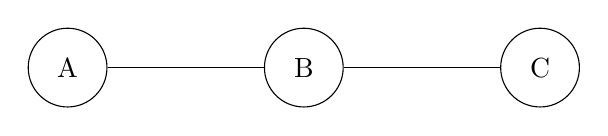
\begin{tikzpicture}
        %%%%%%%%%% Nodi %%%%%%%%%%
        \node[circle, draw, minimum size=1cm] (A) at  (0,0) {A};
        \node[circle, draw, minimum size=1cm] (B) at  (3,0) {B};
        \node[circle, draw, minimum size=1cm] (C) at  (6,0) {C};

        %%%%%%%%% Archi %%%%%%%%%%
        \draw (A) -- (B) -- (C);
    \end{tikzpicture}
\end{center}